%-----Main FIle------
%For Detail check out - http://firesofmay.blogspot.com/2011/10/latex-project-report-template
%CHANGE THESE Settings ONLY IF YOU KNOW WHAT YOU DOING

\documentclass[12pt,a4paper]{report}

%adjust your page margins here
\usepackage[top=0.70in, bottom=0.70in, left=0.8in,right=0.80in]{geometry} % setting the page alignment with this package
\usepackage[pdftex]{graphicx} %for embedding images
%\usepackage[hyphens]{url} %for proper url entries
\usepackage[dvips, bookmarks, colorlinks=false]{hyperref} %for creating links in the pdf version and other additional pdf attributes, no effect on the printed document
\usepackage[final]{pdfpages} %for embedding another pdf, remove if not required
\usepackage{float} %used for figure placement with H as a parameter
%\usepackage[hyphens]{url}
%\usepackage{hyperref}
\usepackage{pslatex} % for times new roman, old package, but works
\usepackage{array} % for making text bold in table


%For inserting Python Code
\usepackage{listings}
\usepackage{color}
 
\definecolor{dkgreen}{rgb}{0,0.6,0}
\definecolor{gray}{rgb}{0.5,0.5,0.5}
\definecolor{mauve}{rgb}{0.58,0,0.82}
 
\lstset{ %
  language=Python,                % the language of the code
  basicstyle=\footnotesize,           % the size of the fonts that are used for the code
  numbers=left,                   % where to put the line-numbers
  numberstyle=\tiny\color{gray},  % the style that is used for the line-numbers
  stepnumber=1,                   % each line is numbered
  numbersep=5pt,                  % how far the line-numbers are from the code
  backgroundcolor=\color{white},      % choose the background color. You must add \usepackage{color}
  showspaces=false,               % show spaces adding particular underscores
  showstringspaces=false,         % underline spaces within strings
  showtabs=false,                 % show tabs within strings adding particular underscores
  frame=single,                   % adds a frame around the code
  rulecolor=\color{black},        % if not set, the frame-color may be changed on line-breaks within not-black text (e.g. commens (green here))
  tabsize=2,                      % sets default tabsize to 2 spaces
  captionpos=b,                   % sets the caption-position to bottom
  breaklines=true,                % sets automatic line breaking
  breakatwhitespace=false,        % sets if automatic breaks should only happen at whitespace
  title=\lstname,                   % show the filename of files included with \lstinputlisting;
                                  % also try caption instead of title
  keywordstyle=\color{blue},          % keyword style
  commentstyle=\color{dkgreen},       % comment style
  stringstyle=\color{mauve},         % string literal style
  escapeinside={\%*}{*)},            % if you want to add a comment within your code
  morekeywords={*,...}               % if you want to add more keywords to the set
}

%%%%For inserting Python Code Over



%For the header and footer
\usepackage{fancyhdr}
\fancypagestyle{plain}{%
%\fancyhf{} % clear all header and footer fields
\fancyfoot[L]{\emph{This project is a Proof of Concept of Social Engineering Attack on Facebook using Web Scraping and Two Man in the middle attack Technique.}} % except the center
\fancyfoot[R]{\thepage}
\renewcommand{\headrulewidth}{0.4pt}
\renewcommand{\footrulewidth}{0.4pt}
}

\pagestyle{fancy}
\lhead{Chapter \thechapter}
\renewcommand{\chaptermark}[1]{% 
\markboth{#1}{}} 

\fancyfoot[LO,LE]{\emph{This project is a Proof of Concept of Social Engineering Attack on Facebook using Web Scraping and Two Man in the middle attack Technique.}}
\cfoot{}
\fancyfoot[RO, RE]{\thepage}
\renewcommand{\headrulewidth}{0.4pt}
\renewcommand{\footrulewidth}{0.4pt}
%For the header and footer Over

% Altering the Index Page Title
%\renewcommand{\contentsname}{\begin{center}\textsc{University Of Pune \\2011 - 2012}\\[1cm]Index\end{center}} 


%GLOBAL SETTINGS OVER, DOCUMENT BEGINS
\begin{document}

%Renames "Bibliography" to "References" on ref page
\renewcommand\bibname{References} 

%FROM HERE YOUR PAGES START GETTING ADDED

% includes the cover page
\thispagestyle{empty}
\begin{center}
    \includegraphics[scale=0.7]{figures/cdut.png}
\end{center}
\vskip1.5cm
\begin{center}
    \makebox[109mm][s]{\heiti\zihao{-0}\bf 本科生实验报告}
\end{center}
\vskip2cm
\begin{center}
    \makebox[20mm][s]{\heiti\zihao{4} 实验课程}\underline{\makebox[130mm][c]{\heiti\zihao{3}\LaTeX 书写行为规范}}\\
    \vskip1cm
    \makebox[20mm][s]{\heiti\zihao{4} 实验名称}\underline{\makebox[130mm][c]{\heiti \zihao{3} 利用\LaTeX 书写成都理工大学实验报告}}\\
    \vskip1cm
    \makebox[20mm][s]{\heiti\zihao{4} 专业名称}\underline{\makebox[130mm][c]{\heiti\zihao{3} 专业全称(有专业方向的用小括号标明)}}\\
    \vskip1cm
    \makebox[20mm][s]{\heiti\zihao{4} 学生姓名}\underline{\makebox[130mm][c]{\heiti\zihao{3} 您的姓名}}\\
    \vskip1cm
    \makebox[20mm][s]{\heiti\zihao{4} 学生学号}\underline{\makebox[130mm][c]{\heiti\zihao{3} 您的学号}}\\
    \vskip1cm
    \makebox[20mm][s]{\heiti\zihao{4} 指导教师}\underline{\makebox[130mm][c]{\heiti\zihao{3} 您的授课或者指导老师}}\\
    \vskip1cm
    \makebox[20mm][s]{\heiti\zihao{4} 实验地点}\underline{\makebox[130mm][c]{\heiti\zihao{3} 授课地点(如:6C403)}}
    \vskip1cm
    \makebox[20mm][s]{\heiti\zihao{4} 实验成绩}\underline{\makebox[130mm][c]{\heiti\zihao{3} 由指导老师书写}}\\
\end{center}
\vskip1.85cm
\vfill\begin{center}
    {\songti\zihao{3}二〇一八年三月二十一日}
\end{center}
\newpage
\thispagestyle{empty}
\tableofcontents
\newpage
\setcounter{page}{1} 
\newpage

% includes the certificate page
%\chapter*{}
\begin{center}
\thispagestyle{empty}

\LARGE{\textbf{Pune Institute of Computer Technology}} \\ 
\large{\textbf{Department of Information Technology}}\\
\large{\textbf{Dhankawadi, Pune – 411043}}\\[0.5cm]

\includegraphics[scale=0.5]{pict_logo}\\[0.5cm]

{\Huge \textbf{\emph{CERTIFICATE}}}\\[0.5cm]
\end{center}
\linespread{1.13}
\large{This is certify that the Dissertation entitled 
\textbf{``PROJECT NAME'',} 
submitted by 
\textbf{YOUR NAME}
 is a record of bonafide work carried out by him, in the partial
 fulfilment of the requirement for the award of Degree of Bachelor of
 Engineering (Information Technology) at Pune Institute of Computer
 Technology, Pune under the University of Pune. This work is done
 during year 2011-2012, under our guidance.}\\[1.0cm]
\large{---------------------------------}\\
\large{(Prof. GUIDES NAME)}\\[0.3cm]
\textbf{Project Guide}\\[1.0cm]
\large{--------------------------------}\hspace*{1.5in}\large{----------------------------------}\\
\large{Prof. Emmanual M.}\hspace*{2.0in}\large{Dr. P. T. Kulkarni}\\[0.3cm]
\textbf{HOD, IT Department}\hspace*{1.73in}\textbf{Principal PICT}\\[0.5cm]
\Large{\textbf{Examination:}}\\[0.8cm]
\large{Examiner ------------------------}\\[0.8cm]
\Large{\textbf{Date:}}
\newpage
 
\newpage

% includes the acknowledgements page
\documentclass[../thesis.tex]{subfiles} % so that this document can be compiled on its own

\begin{document}

\begin{danksagung*}
\todo{Ihr Text hier.}
\end{danksagung*}

\begin{acknowledgements*}
\todo{Enter your text here.}
\end{acknowledgements*}

\end{document} 
\newpage

% includes the company 	certificate page
%\chapter*{}
\begin{center}
\thispagestyle{empty}
\vspace*{4\baselineskip}
\LARGE{\textbf{CERTIFICATE}}\\[1.0cm]
\large{This is to certify that the project report entitled}\\[0.7cm]
\Large{\textbf{PROJECT NAME}}\\[0.7cm]
\normalsize{Submitted by}\\[0.3cm]
\end{center}
\begin{table}[h]\large
\centering
\begin{tabular}{>{\bfseries}lc>{\bfseries}r}
XXXXXXX & & B1231414\\ %Example B-1231414
YYYYYYY & & B1231414\\ %Example B-1231414
ZZZZZZZ & & B1231414\\ %Example B-1231414
\end{tabular}
\end{table}
\normalsize{is a bonafide work carried out by them with the Sponsorship from ------------------- under the
\\supervision of Mr. ................................ and has been completed successfully .}\\[1.5cm]
\normalsize{(Mr. .................. )}\\
\normalsize{(Designation)}\\
\normalsize{External Guide}\\[1cm]
\normalsize{Place : Pune}\\
\normalsize{Date:}\\
\newpage
 
\newpage

%# -*- coding: utf-8-unix -*-
%%==================================================

\begin{abstract}
本项目为年产50万吨MTO工厂的初步设计。通过分析当前国内外MTO生产和研究现状,对生产工艺进行了选择论证。然后运用Aspen软件模拟初步的工艺流程,并通过对一系列工艺参数,如精馏塔的塔板数—产品纯度、进料塔板数—产品纯度、产品纯度—回流比、再沸器负荷—回流比等进行灵敏度分析,优化设备操作条件,提高工艺的合理性和经济性。本设计还针对工艺流程进行换热网络设计和对全局换热网络进行了优化和评估,通过内部流股之间相互换热以减少公用工程的消耗,最终优化后节约$79.4\%$的热公用工程资源和$73.7\%$的冷公用工程资源。本设计还运用水夹点技术优化了用水网络,根据水硬度分类处理水操作单元,并合理再生利用,使得本项目新鲜水用量和废水排放量达到最小,优化后的用水网络节约用水$53.59\%$。本设计对于MTO工厂的生产和设计建造具有一定的现实指导意义。\\

\keywords{\zihao{-4} 工厂\quad 设计\quad MTO \quad 工艺 \quad 水夹点  \quad 网络 \quad 控制}
\end{abstract}

\begin{englishabstract}

This project is the preliminary design of a MTO plant with an annual output of 500,000 tons of light olefins. Based on the current production and research situation all through the world, the production method was selected and demonstrated. Aspen software was used to simulate the preliminary process. Heat integration method was applied to optimize the heat exchange network. Rational heat exchange between process streams were suggested which resulted in the decreasing of utilities consumption and exchanger number. The heat integration leaded to energy saving of $79.4\%$ of heat utilities and $73.7\%$ of the cold utilities. In addition, the water pinch technology was also implemented to optimize the water network. The water operating unit was classified according to water hardness, with a reasonable recycling. The amount of fresh water consumption and wastewater emission was minimized. The optimized water network achieved $53.59\%$ water saving. Finally, a preliminary economic analysis to the entire project was estimated in order to get the project construction cost and profitability. In summary, this design is of some practical significance for the production and design of the MTO industry.

\englishkeywords{\zihao{-4} Plant design\;Sensitivity analysis  \; Energy balance\; calculation \; Water pinch  Dynamic control}
\end{englishabstract}

 % adds the Research Methodology page
\newpage

%TABLE OF CONTENTS AND LIST OF FIGURES ARE AUTOMATICALLY ADDED BY FOLLOWING COMMANDS
%ADD FIGURE OF TABLES IF YOU NEED TO, CHECK DOCUMENTATION
\pagenumbering{roman} %numbering before main content starts


%To reset the Header & Footer for TOC and LOF
\pagestyle{empty}
\addtocontents{toc}{\protect\thispagestyle{empty}}
\tableofcontents % adds Index Page

%\pagestyle{empty}

\addtocontents{lof}{\protect\thispagestyle{empty}}
\listoffigures % adds List of Figures
\cleardoublepage

%And reset back the settings we choose for Header and Footer
\pagestyle{fancy}

\newpage
\pagenumbering{arabic} %reset numbering to normal for the main content


\lettrine[lines=3]{T}{he MC methodology} mainly considers two types of point-based temporal logics (PTLs) as the property specification language---\emph{linear} and \emph{branching}---which differ 
in the underlying model of time.
In linear PTLs, such as $\LTL$~\cite{Pnu77}, each moment in time has a unique possible future:
formulas are interpreted over (infinite) \emph{paths} of a Kripke structure, and thus they refer to a single computation of a system.
In branching PTLs,
such as $\CTL$ and $\CTLStar$~\cite{EH86}, each moment in time may evolve into several possible futures:
formulas are interpreted over \emph{states} of the Kripke structure, hence referring to all the possible system computations.

In the previous chapters we have assumed a \emph{state-based} semantics for $\HS$, which
induces a branching reference both in the future and in the past:
intervals/traces 
are \lq\lq forgetful\rq\rq{} of the history leading to their initial state, and  
the initial (resp., final) state of an interval may feature several predecessors (resp., successors).
A graphical account of the state-based semantics can be found in Figure~\ref{fig:ST}; a detailed explanation will be given in the following.

\begin{figure}[tp]
\centering
\begin{minipage}{0.36\linewidth}
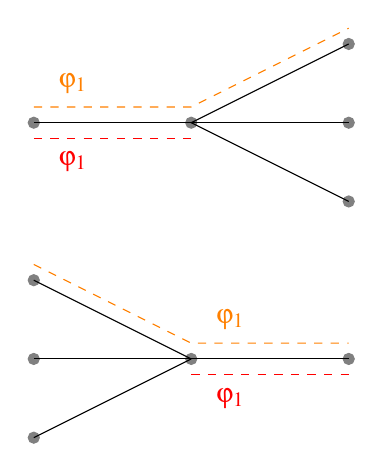
\begin{tikzpicture}
				%				[->,>=stealth',shorten >=1pt,auto,node distance=0,main node/.style={circle,draw}]
				\filldraw [gray] (0,2) circle (2pt)
				(2,2) circle (2pt)
				(4,3) circle (2pt)
				(4,2) circle (2pt)
				(4,1) circle (2pt);
				%
					\filldraw [gray] (4,-1) circle (2pt)
				(2,-1) circle (2pt)
				(0,0) circle (2pt)
				(0,-1) circle (2pt)
				(0,-2) circle (2pt);
				%
				\draw [black]  (0,2) -- (4,2);
				\draw [black]  (0,-1) -- (4,-1);
				%
				\draw [black] (2,2) -- (4,3);
				\draw [black] (2,2) -- (4,1);
				\draw [black] (0,0) -- (2,-1);
				\draw [black] (0,-2) -- (2,-1);
				%
				\draw [dashed, orange] (0,2.2) -> (2,2.2) -> (4,3.2);
				\draw [dashed, red] (0,1.8) -> (2,1.8);
				\draw [dashed, orange] (0,0.2) -> (2,-0.8) -> (4,-0.8);
				\draw [dashed, red] (2,-1.2) -> (4,-1.2);
				
	%		{\tiny
				\node [orange] at (0.5,2.5) {$\varphi_1$};	
				\node [red] at (0.5,1.5) {$\hsBt\varphi_1$};
			\node [orange] at (2.5,-0.5) {$\varphi_1$};	
				\node [red] at (2.5,-1.5) {$\hsEt\varphi_1$};
		%			\node (b0) at (4,-0.5) {$\rho'=\rho(0,i)\cdot \rho^{(j+1)]}$};	
		%			\node (a1) at (1.5,0.2) {$\rho(i)=$};
		%			\node (a2) at (2,0.2) {$\rho(j)$};
		%			\node (a3) at (1.65,0.5) {$Pattern(\rho,i)= Pattern(\rho,j)$};
		%			\node (a4) at (4.6,0.5) {$Pattern(\rho,k) =\{ p \in \Prop : \Ku,\rho^{k]} \models p\}$};
						
	%			}
				
			\end{tikzpicture}
\end{minipage}	
\hfill 	
\begin{minipage}{0.54\linewidth}
			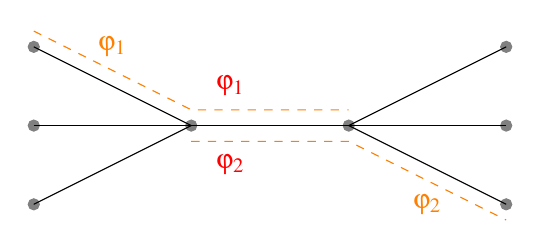
\begin{tikzpicture}
				%				[->,>=stealth',shorten >=1pt,auto,node distance=0,main node/.style={circle,draw}]
				%
					\filldraw [gray] (4,-1) circle (2pt)
				(2,-1) circle (2pt)
				(0,0) circle (2pt)
				(0,-1) circle (2pt)
				(0,-2) circle (2pt)
				(6,0) circle (2pt)
				(6,-1) circle (2pt)
				(6,-2) circle (2pt)	;
				%
				\draw [black]  (0,-1) -- (6,-1);
				%
				\draw [black] (4,-1) -- (6,0);
				\draw [black] (4,-1) -- (6,-2);
					\draw [black] (0,0) -- (2,-1);
				\draw [black] (0,-2) -- (2,-1);
				%
				\draw [dashed, orange] (0,0.2) -> (2,-0.8) -> (4,-0.8);
				\draw [dashed, orange] (2,-1.2) -> (4,-1.2) -> (6,-2.2);
				
	%		{\tiny
				\node [orange] at (1,0) {$\varphi_1$};	
				\node [red] at (2.5,-0.5) {$\hsAt\varphi_1$};
			\node [orange] at (5,-2) {$\varphi_2$};	
				\node [red] at (2.5,-1.5) {$\hsA \varphi_2$};
		%			\node (b0) at (4,-0.5) {$\rho'=\rho(0,i)\cdot \rho^{(j+1)]}$};	
		%			\node (a1) at (1.5,0.2) {$\rho(i)=$};
		%			\node (a2) at (2,0.2) {$\rho(j)$};
		%			\node (a3) at (1.65,0.5) {$Pattern(\rho,i)= Pattern(\rho,j)$};
		%			\node (a4) at (4.6,0.5) {$Pattern(\rho,k) =\{ p \in \Prop : \Ku,\rho^{k]} \models p\}$};
						
	%			}
				
			\end{tikzpicture}
\end{minipage}
%
    \caption{State-based semantic variant $\HS_\stat$: past and future are branching}
    \label{fig:ST}
\end{figure}

However, as we already said, $\HS$ MC has been simultaneously and independently studied also by Lomuscio and Michaliszyn in~\cite{LM13,LM14,lm16}:
there, the considered $\HS$ fragments are interpreted over the unwinding of a Kripke structure (\emph{computation-tree-based} semantics---see Figure~\ref{fig:CT}). %, and interval labeling takes into account only the endpoints of intervals. 
This induces a linear reference in the past (the initial state of an interval may feature only one predecessor), but branching in the future (the final state features several successors). Moreover, the computation history is never forgotten and increases with time.

\input{Chaps/TOCL17/Imgs/semPicturesCT.tex}

In this chapter, we study the expressiveness of $\HS$, in the context of MC, in comparison with that of the standard PTLs $\LTL$, $\CTL$, and $\CTLStar$. The analysis is carried on \emph{enforcing the homogeneity assumption}.
% 
We prove that $\HS$ endowed with the state-based semantics (hereafter denoted as $\HS_\stat$) is not comparable with $\LTL$, $\CTL$, and $\CTLStar$. On one hand, the result supports the intuition that $\HS_\stat$ gains some expressiveness by the ability of branching in the past. On the other hand, $\HS_\stat$ does not feature the possibility of forcing the verification of a property over an %linear 
infinite path, thus implying that the formalisms are not comparable. With the aim of having a more ``effective'' comparison base, we consider two additional semantic variants of $\HS$, 
%besides the state-based one $\HS_\stat$, 
namely, the \emph{computation-tree-based semantic variant} (denoted as $\HS_\LinearPast$) and the \emph{trace-based} one ($\HS_\LinearTime$). 
\input{Chaps/TOCL17/Imgs/semPicturesLN.tex}

The state-based (see Figure~\ref{fig:ST}) and computation-tree-based (see Figure~\ref{fig:CT}) approaches rely on a \emph{branching}-time setting and differ in the nature of past. In the latter approach, past is \emph{linear}: each interval may have several possible futures, but only a unique past. Moreover, past is assumed to be \emph{finite} 
%(since program computations have a definite starting time) 
and \emph{cumulative}, that is, the story of the current situation increases with time, and is never forgotten. 
%
%Finally, the 
The trace-based approach relies on a \emph{linear}-time setting (see Figure~\ref{fig:LN}), where the infinite paths (computations) of the given Kripke structure are the main semantic entities. Branching is neither allowed in the past nor in the future.
%
Note that the linear-past (rather than branching) approach is more suited to the specification  of dynamic behaviors, because it considers states in a computation tree, while the branching-past approach considers machine states, where past is not very meaningful for the specification of behavioral constraints~\cite{LS95}.

The variant $\HS_\LinearPast$ is a natural candidate for an expressiveness comparison with the branching time logics  $\CTL$ and $\CTLStar$. The most interesting and technically involved result is the characterization of the expressive power of $\HS_\LinearPast$: $\HS_\LinearPast$ turns out to be expressively equivalent to finitary $\CTLStar$, that is, the variant of $\CTLStar$ with quantification over \emph{finite} paths. As for $\CTL$, a non comparability result can be stated.
%
%Conversely, 
The variant $\HS_\LinearTime$ is a natural candidate for an expressiveness comparison with $\LTL$: 
%As a matter of fact, 
we prove that $\HS_\LinearTime$ and $\LTL$ are equivalent (this result holds true even for a very small fragment of $\HS_\LinearTime$), but the former is at least exponentially more succinct than the latter. 

We complete the picture with a comparison of the three semantic variants $\HS_\stat$, $\HS_\LinearPast$, and $\HS_\LinearTime$. We show that, as expected, $\HS_\LinearTime$ is not comparable with either of the branching versions, $\HS_\LinearPast$ and $\HS_\stat$. The interesting result is that, on the other hand, $\HS_\LinearPast$ is strictly included in $\HS_\stat$: this supports $\HS_\stat$ as a reasonable and adequate semantic choice.

\begin{figure}[b]
%\vspace*{-0.4cm}
\centering
%\resizebox{\width}{\height}{%
\begin{tikzpicture}[-,>=stealth',shorten >=1pt,auto,semithick,main node/.style={rectangle,draw,inner sep=2pt}]  
%
\tikzstyle{gray node}=[fill=gray!30]
%
\node [main node](0) at (0,0) {$\HS_\LinearPast$};
\node [main node](1) at (0,1.5) {$\HS_\LinearTime$};
\node [main node](2) at (0,-1.5) {$\HS_\stat$};
\node [main node](3) at (2.5,0) {finitary $\CTLStar$};
\node [main node](4) at (2.5,1.5) {$\LTL$};
\node [main node](6) at (2.5,-1.5) {$\CTL$};
\node [main node](5) at (5,0) {$\CTLStar$};
%   
\draw [dashed] (0.east) to node {$\equiv$} (3);
\draw [dashed] (1.east) to node {$\equiv$} (4);
\draw [dashed] (3.east) to node {$<$} (5);
\draw [dashed] (0.north) to node [swap] {$\neq$} (1);
\draw [dashed] (0.south) to node {\rotatebox{-90}{$<$}} (2);
\draw [dashed] (2.east) to node [swap] {$\neq$} (6.west);
\draw [dashed] (2) [out=-40,in=270] to node [near end] {$\neq$} (5);
\draw [dashed] (0.south east) to node {$\neq$} (6.west);
\draw [dashed] (2) [out=135,in=225] to node {$\neq$} (1);
\end{tikzpicture}%}
\vspace*{-0.6cm}
\caption{Overview of the expressiveness results.}\label{results}
\end{figure}

The complete picture of the expressiveness results is reported in Figure~\ref{results}
(the symbols $\neq$, $\equiv$, and $<$ denote incomparability, equivalence, and strict %expressiveness 
inclusion, respectively).

\paragraph*{Organization of the chapter.}
\begin{itemize}
	\item In the next section we start with some preliminaries; in particular, in Section~\ref{sect:PTL} we recall the well-known PTLs $\LTL$, $\CTL$ and $\CTLStar$; in Section~\ref{sect:3sem} we define the three semantic variants of $\HS$ ($\HS_\stat$, $\HS_\LinearPast$ and $\HS_\LinearTime$). In Section~\ref{subs:vendingMach} we provide a detailed example which gives an intuitive account of the three semantic variants and highlights their differences.
	\item In the next three sections we analyze and compare the expressiveness of these logics.  
In Section~\ref{sec:CharacterizezionOfLeniarTimeHS} we show the expressive equivalence of $\LTL$ and $\HS_\LinearTime$. Then, in Section~\ref{sec:characterizationHSLinearPast} we prove the equivalence of $\HS_\LinearPast$ and finitary $\CTLStar$. In Section~\ref{sect:allSems} we compare the expressiveness of 
$\HS_\stat$, $\HS_\LinearPast$ and $\HS_\LinearTime$.
\end{itemize}
 % adds the introduction page
\chapter{Literature Survey}

\section{Paper1}

\subsection{Summary}

XXXXXXX

\subsection{Advantages}

XXXXXXX
\subsection{Disadvantages}

XXXXXXX % adds the Literatu	re Survey page
\chapter{Proposed Work}

\section{Problem Statement}
XXXXXXX

\section{Module1}
XXXXXXX
\subsection{SubSection1}
XXXXXXX % adds the Project Work page
\chapter{Research Methodology}

\section{Module1}

\subsection{Subsection}
XXXXXXX
\subsubsection{SubSub}
XXXXXXXXXXXXXXXXXXXXX     % adds the Research Methodology page
\input{project-design.tex} % adds the Project Design
\chapter{Implementation}

\section{Module1}

\subsection{Submodule1}
Code Snippet
\lstinputlisting{helloworld.py}
XXXXXXXXXXXXXXXXXXXXX % adds the Project Design
\chapter{Scheduling}


\section{Proposed Modules}

XXXXXXX
\section{Scheduling}

XXXXXXX % adds the Scheduling and Planning page
\chapter{Conclusion and Future Scope}


\section{Future Scope}



\section{Conclusion}

 % adds the Scheduling and Planning page
\begin{thebibliography}{99}
\addcontentsline{toc}{chapter}{\bibname}
\lhead{}\markboth{\bibname}{}

% \bibitem{TEXT} is how you refer to your reference in your report. keep that very short
% \emph{Paper Name} is just to highligh the paper name by making it italic, not required but looks nice

%Example
%\bibitem{short_paper_name}\emph{Paper Name}; Author Name, Conference Name, year etc 


%And how you would refer to the paper in the text - example
%Your text in other tex files \cite{short_paper_name} contd explaining

%If you have to display links, do it via  adding \\ (newline) otherwise it goes off the margins. Don't know how to fix this yet
%\bibitem{short_link_name}Link Name \\ \url{http://url link here}
%\url{The-human-element-the-weakest}



\end{thebibliography} % adds the References page

\end{document}
